%        File: FireflySpec_1p0.tex
%     Created: Thu Jan 17 01:00 PM 2019 E
%
\documentclass[letterpaper,11pt]{article}
\usepackage[leqno]{amsmath}
\usepackage{mathptmx,courier}
\usepackage[scaled]{helvet}
\usepackage[inter-unit-product=\ensuremath{{}\cdot{}},per-mode=symbol,separate-uncertainty,binary-units]{siunitx}
\usepackage[letterpaper,lmargin=0.75in,rmargin=0.75in,tmargin=0.75in,bmargin=1.00in]{geometry}
\usepackage{paralist}
%\usepackage{alltt}
\usepackage{supertabular}
\usepackage[pdftex]{graphicx}
\usepackage[hyperfigures=false,bookmarks=false,pdftex,colorlinks,linkcolor=black,urlcolor=blue]{hyperref}
\usepackage[cachedir=/home/kjh016/tmp/mintedcache]{minted}

\graphicspath{{graphics/}}

\ifpdf\pdfinfo{
  /Title (Firefly Simulator Specification) %FIXME
  /Author (Bucknell University) %FIXME
/Keywords () }
\fi

% load hyperref package first!!
\usepackage{fancyhdr,pageslts}
\pagestyle{fancy}
\fancyhf{}
\fancyhead[L]{Firefly Simulator Specification V2.1}   %FIXME
\fancyfoot[C]{Page \thepage\ of \pageref*{LastPage}}
\usepackage[iso]{datetime}
\fancyfoot[L]{Revised \today}
\pagenumbering{arabic}
\renewcommand\headrulewidth{0pt}

\begin{document}
\section{Overview}

This document provides specifications for a \textit{firefly simulator}. This
device is intended to simulate the light displays of common fireflies, such
as \textit{Photinus pyralis}. The \textit{firefly simulator} will provide means
to control the brightness, duration, and other relevant parameters of the
simulated light display. Light-emitting diodes (LEDs) will be used as the light
source, and the color of the display can be altered by connecting different
LED types to the simulator.

The \textit{firefly simulator} can be configured via commands issued to it
from a host computer, as shown in Fig.\ \ref{fig:BlockDiagram}. The physical
link between the host computer and the \textit{firefly simulator} is an
asynchronous serial communications interface, which can be accomplished with a
common and inexpensive USB adapter. The \textit{firefly simulator} also can
return status information to the host computer via the same interface.

Once configured, the \textit{firefly simulator} can be used in a stand-alone
mode, without requiring a connection to a host computer. Pushbuttons on the
\textit{firefly simulator} can be used to activate light displays that were
previously configured. When in the stand-alone mode, the simulator can be
powered by a USB powerbank.

\begin{figure}[h]
  \begin{center}
    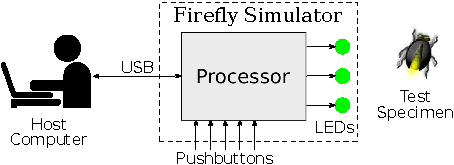
\includegraphics[scale=1.5]{Flashes_BlockDiagram}
  \end{center}
  \vspace{-18pt}
  \caption{Firefly Simulator Block Diagram}
  \label{fig:BlockDiagram}
\end{figure}

This document describes the minimum required functionality of the
\textit{firefly simulator}. Possible future enhancements to the simulator
include:
\begin{compactitem}
  \item The ability to sense the behavior of a test specimen and use that
    behavior to modify the parameters of a light display.
  \item The ability to record information about simulator activity on
    non-volatile memory, such as a removable Secure Digital (SD) memory card.
\end{compactitem}

\section{References}

\begin{enumerate}
  \item 
\textit{IEEE Standard for Transitions, Pulses, and Related Waveforms},
  IEEE Standard 181, 2011.
  \item 
\textit{Data elements and interchange formats – Information
interchange – Representation of dates and times}, ISO 8601
\end{enumerate}


\section{Definitions}

\begin{figure}[h]
  \begin{center}
    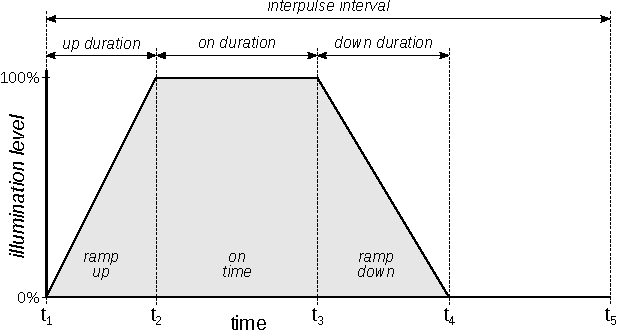
\includegraphics{Flashes_FlashPulse}
  \end{center}
  \vspace{-18pt}
  \caption{\textit{flash} waveform}
  \label{fig:FlashPulse}
\end{figure}

\setlength\extrarowheight{4pt}
\begin{supertabular}{p{1.25in}p{5.25in}}
abort &
    A pushbutton input to the \textit{firefly simulator}. Pressing this button
    causes the simulator to stop any repeated \textit{flashes} or
    \textit{patterns}, and to bring the \textit{illumination level} to 0\% on
    all \textit{channels}.\\
ASCII &
    The American Standard Code for Information Interchange. The letters in
    the English alphabet, the decimal digits, and common punctuation marks are
    assigned a unique 7-bit binary code.\\
channel &
    The \textit{channel} of an \textit{LED} is an integer that specifies
    which physical output connector of the firefly simulator is connected
    to the physical LED. The value of \textit{channel} is an integer and
    shall not be less than 1 and not greater than \textit{max channel}.\\
        &
    Note that the \textit{channel} is not the pin number of any particular
    microcontroller. An implementation of the firefly simulator must perform
    the appropriate mapping of an \textit{LED}'s \textit{channel} to an
    appropriate physical pin on the output device.\\
%delay step&
%    A time interval in a \textit{pattern} when all \textit{LEDs} are dark.
%    A \textit{delay step} is a step in a \textit{pattern} that inserts a time
%    delay but does not cause a flash.\\
down duration & 
    The length of the \textit{ramp down} interval. The \textit{down duration}
    is equal to $t_4 - t_3$, as shown in Fig.\ \ref{fig:FlashPulse}. The
    \textit{down duration} shall be a non-negative integer value with units
    of milliseconds. The value of \textit{down duration} shall not be less
    than 0 or greater than 32\,767.\\
%duty factor &  For a periodic rectangular pulse that has only two possible
%    voltage levels, the \textit{duty factor} is the ratio of the duration of
%    the pulse at its higher voltage divided by the period of the waveform.
%
%    \[ 0.0 \le d_f \le 1.0 \quad \mathrm{ or } \quad 0\% \le d_f \le 100\%\]
event &
    An external event that can be recognized by the \textit{firefly simulator}.
    Details TBD.\\
flash &
    The process of bringing the \textit{illumination level} of an \textit{LED}
    from 0\% to 100\% then back to 0\% illumination. A \textit{flash} consists of
    a \textit{ramp up}, followed by an \textit{on time}, followed by a
    \textit{ramp down}. A \textit{flash} begins at $t_1$ and ends at $t_4$,
    as shown in Fig.\ \ref{fig:FlashPulse}. The interval from $t_1$ to $t_2$
    is the \textit{ramp up}. The interval from $t_2$ to $t_3$ is the \textit{on
    time}.  The interval from $t_3$ to $t_4$ is the \textit{ramp down}. The
    interval from $t_4$ to $t_5$ is the \textit{interpulse interval}.\\
    &
    Note the definition of a \textit{flash} primarily specifies the
    \textit{timing} behavior of the \textit{flash}. The selection of a specific
    physical LED and its \textit{max brightness} are part of the definition
    of an \textit{LED}.\\
flash pattern interval &
    The total time duration of a \textit{pattern}.
    This interval includes the time of all \textit{flashes} in the pattern
    as well as the subsequent time when there are no flashes, as shown in
    Fig.\ \ref{fig:PatternTimeline}. The
    \textit{flash pattern interval} is a parameter of a \textit{pattern}.\\
illumination level &
    The brightness of an \textit{LED} at any given point in time, as a
    percentage of that \textit{LED}'s \textit{max brightness}. The
    \textit{illumination level} and \textit{max brightness} values
    indirectly translate to the average current passing through the physical
    LED.\\
    &
    At any given point in time, the average current for an LED is
\[ I_{AVG} = \frac{illumination\,level}{100} \times \frac{max\,brightness}{100}
\times I_{max}\]\\
interpulse interval &
    The total time duration of a \textit{flash}. This interval includes the
    time when the \textit{LED} is illuminated as well as the subsequent time
    when the \textit{LED} is not illuminated, from $t_1$ to $t_5$ in
    Fig.\ \ref{fig:FlashPulse}. The \textit{interpulse interval} is a parameter
    of a \textit{flash}.\\
message &  A sequence of \textit{message fields}, separated by the
    ASCII comma character (decimal 44) and terminated by either the ASCII Line
    Feed (decimal 10), the ASCII Carriage Return (decimal 13), or both the Line
    Feed and the Carriage Return. There shall not be a comma before the first
    field in a message nor after the last field.\\
message field &  A sequence of one or more ASCII characters from the set of
    letters (\texttt{A} through \texttt{Z} and \texttt{a} through \texttt{z}),
    decimal digits (\texttt{0} through \texttt{9}), and the punctuation
    characters required for a \textit{timestamp} (colon, minus, plus, period).
    A message field shall not include a comma.\\
max brightness & 
    The maximum duty factor of the \textit{pulse-width modulation} signal that
    controls the \textit{illumination level} of an \textit{LED}. The
    \textit{max brightness} is a characteristic of an \textit{LED}. The
    value of \textit{max brightness} is an integer and shall be not less
    than 1 and not greater than 100.\\
max channel & 
    The number of physical \textit{LED} \textit{channels} available on a
    particular implementation of a \textit{firefly simulator}.
    The value of \textit{max channel} shall not be less than 1 or greater
    than 127 for any implementation of a \textit{firefly simulator}.\\
max event &
    The number of unique \textit{event} configurations available on a
    particular implementation of a \textit{firefly simulator}.
    The value of \textit{max event} shall not be less than 0 or greater
    than 127 for any implementation of a \textit{firefly simulator}.\\
max flash & 
    The number of unique \textit{flash} configurations available on a
    particular implementation of a \textit{firefly simulator}.
    The value of \textit{max flash} shall not be less than 1 or greater
    than 127 for any implementation of a \textit{firefly simulator}.\\
max LED & 
    The number of unique \textit{LED} configurations available on a
    particular implementation of a \textit{firefly simulator}.
    The value of \textit{max LED} shall not be less than 1 or greater
    than 127 for any implementation of a \textit{firefly simulator}.\\
max pattern & 
    The number of unique \textit{pattern} configurations available on a
    particular implementation of a \textit{firefly simulator}.
    The value of \textit{max pattern} shall not be less than 1 or greater
    than 127 for any implementation of a \textit{firefly simulator}.\\
on duration &
    The length of the \textit{on time} interval. The \textit{on duration} is
    equal to $t_3 - t_2$, as shown in Fig.\ \ref{fig:FlashPulse}. The value
    of \textit{on duration} shall be a positive, non-zero integer with units
    of milliseconds. The value of \textit{on duration} shall not be less than 1
    or greater than 32\,767.\\
on time &
    The period of time during a \textit{flash} when the \textit{LED} is
    constantly at an illumination level of 100\%.\\
pattern &
    A sequence of up to 16 \textit{flashes}, possibly followed by a period
    of time where there are no \textit{flashes}.
    Note that the definition of a \textit{pattern} specifies only the sequence
    of \textit{flashes} that should occur as well as the total duration of the
    \textit{pattern}.\\
%pulse-width modulation & 
ramp down &
    The process of linearly decreasing the \textit{illumination level} of an
    \textit{LED} from 100\% to 0\%.\\
ramp up &
    The process of linearly increasing the \textit{illumination level} of an
    \textit{LED} from 0\% to 100\%.\\
time stamp &
    A representation of the current date and time used as a \textit{message
    field}. The \textit{time stamp} shall conform to ISO 8601. The format of
    the \textit{time stamp} is \texttt{YYYY-MM-DDTHH:MM:SSZ}. The `\texttt{-}'
    character delimits the year, month, and day fields; the `\texttt{T}'
    delimits the date from the time; the `\texttt{:}' character delimits the
    hours, minutes, and seconds fields. All time values are reported using
    24-hour UTC (Zulu) time rather than the local timezone.\\
up duration &
    The length of the \textit{ramp up} interval. The \textit{up duration}
    is equal to $t_2 - t_1$, as shown in Fig.\ \ref{fig:FlashPulse}. The
    value of \textit{up duration} shall be a non-negative integer with units
    of milliseconds. The value of \textit{up duration} shall not be less than
    0 or greater than 32\,767.\\
\end{supertabular}

\begin{figure}[t]
  \begin{center}
    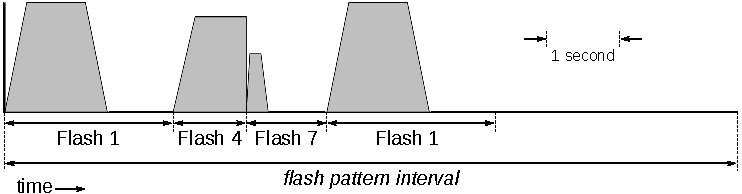
\includegraphics[scale=1.2]{Flashes_PatternTimeline2}
  \end{center}
  \vspace{-18pt}
  \caption{Example \textit{pattern} timeline}
  \label{fig:PatternTimeline}
\end{figure}

\section{Resolution and Accuracy}

\subsection{Brightness}

The \textit{firefly simulator} does not directly control the brightness of a
physical LED. Instead, the simulator controls the average current provided to
the LED. The simulator's configuration messages allow the actual average
current ($I_{AVG}$) of an LED to be specified with a resolution of $\pm 1$\% of
the maximum available current ($I_{MAX}$). The maximum available current, and
the precision which with the current can be specified, will be
determined by the circuitry associated with a given physical LED and need not be
the same for all LEDs.

\subsection{Time}

Values that represent time shall have units of milliseconds and a resolution
of \SI{1}{\milli\second}. The accuracy of all pulse durations and time delays
generated by the \textit{firefly simulator} over an \textit{interpulse interval}
shall have a maximum error of \SI{\pm 10}{\milli\second}. The cumulative timing
error over a \textit{flash pattern interval} shall not exceed
\SI{200}{\milli\second}.

\section{Configuration Messages}

The firefly simulator is configured via a serial communications interface to
a host computer. The host computer can set the values of all parameters for
\textit{LEDs}, \textit{flashes}, and \textit{patterns}. A unique configuration
message format is specified for configuring an \textit{LED}, configuring a
\textit{flash}, or configuring a \textit{pattern}.

\subsection{\textit{LED Configuration Message}}

An \textit{LED Configuration Message} is sent from the host computer to the
firefly simulator. Every \textit{LED Configuration Message} shall contain
four \textit{message fields}, as shown in Table \ref{tab:LEDConfig}.

As an example, the three messages below could be sent by the host computer in
order to configure three \textit{LEDs}.
This example assumes that \textit{LED} 2 uses physical \textit{channel}
1 and has a \textit{max brightness} of 100\%. \textit{LEDs} 3 and 5 use the
same physical \textit{channel} (i.e.\ the same physical LED) but with different
levels of \textit{max brightness}: 87\% and 53\%, respectively.
The \textit{LED} numbers, \textit{channel} numbers, and \textit{max brightness}
levels shown here were chosen
arbitrarily; the purpose of this example is only to illustrate the syntax of
the \textit{LED Configuration Message}.\\[12pt]
{\ttfamily
L,2,1,100\\
L,3,6,87\\
L,5,6,53\\
}

\begin{table}[H]
  \caption{Definition of the \textit{LED Configuration Message}}
  \centering
  \setlength\extrarowheight{2pt}
  \begin{tabular}[h]{|p{0.5in}|p{1.00in}|p{2.25in}|p{2.25in}|} \hline
    Field Number & Field Name & Description & Format \\ \hline
    1            & Header
    & Unique first character for an \textit{LED Configuration Message}
    & This field shall be the uppercase letter `\texttt{L}'.
    \\ \hline
    2            & \textit{LED} number
    & A unique identifier for each \textit{LED} definition
    & This field shall contain a decimal integer from 1 to \textit{max LED}.
    \\ \hline
    3            & LED \textit{channel}
    & The physical channel associated with this \textit{LED}
    & This field shall contain a decimal integer from 1 to \textit{max channel}.
    \\ \hline
    4            & \textit{max brightness}
    & The maximum brightness level for the \textit{LED}
    & This field shall contain a decimal integer from 1 to 100.
    \\ \hline
  \end{tabular}
  \label{tab:LEDConfig}
\end{table}

\subsection{\textit{Flash Configuration Message}}

A \textit{Flash Configuration Message} is sent from the host computer to the
firefly simulator. This message provides the parameters for a single
\textit{flash} of an \textit{LED}, as shown in Table \ref{tab:FlashConfig}.

As an example, the three messages below could be sent by the host computer in
order to configure the three \textit{flashes} shown in Fig.\
\ref{fig:PatternTimeline}. This example assumes that \textit{flash} 1 uses
\textit{LED} 2, \textit{flash} 4 uses \textit{LED} 3, and \textit{flash} 7 uses
\textit{LED} 5. The \textit{flash} and \textit{LED} numbers were chosen
arbitrarily; the purpose of this example is only to illustrate the syntax of
the \textit{Flash Configuration Message}.\\[12pt]
{\ttfamily
F,1,2,300,800,300,2300\\
F,4,3,300,700,0,1000\\
F,7,5,50,150,100,1100\\
}

\begin{table}[h]
\centering
\caption{Definition of the \textit{Flash Configuration Message}}
\label{tab:FlashConfig}
\setlength\extrarowheight{2pt}
\begin{tabular}[h]{|p{0.5in}|p{1.00in}|p{2.25in}|p{2.25in}|} \hline
Field Number & Field Name & Description & Format \\ \hline
1            & Header
             & Unique first character for a \textit{Flash Configuration Message}
             & This field shall be the uppercase letter `\texttt{F}'.
             \\ \hline
2            & \textit{flash} number
             & A unique identifier for each \textit{flash} definition
             & This field shall contain a decimal integer from 1 to
             \textit{max flash}.
             \\ \hline
3            & LED number
             & Identifier for the \textit{LED} to be illuminated in this
             \textit{flash}
             & This field shall contain a decimal integer from 1 to
             \textit{max channel}.
             \\ \hline
4            & \textit{up duration}
             & The duration of the \textit{ramp up} in milliseconds
             & This field shall contain a decimal integer from 0 to 32\,767.
             \\ \hline
5            & \textit{on duration}
             & The duration of the \textit{on time} in milliseconds
             & This field shall contain a decimal integer from 1 to 32\,767.
             \\ \hline
6            & \textit{down duration}
             & The duration of the \textit{ramp down} in milliseconds
             & This field shall contain a decimal integer from 0 to 32\,767.
             \\ \hline
7            & \textit{interpulse interval}
             & The duration of the entire \textit{flash} in milliseconds
             & This field shall contain a decimal integer from 0 to 32\,767.
             \\ \hline
\end{tabular}
\end{table}

\subsection{\textit{Pattern Configuration Message}}

A \textit{Pattern Configuration Message} is sent from the host computer to the
firefly simulator. This message provides the parameters for a single
\textit{pattern} of one or more \textit{flashes}, as shown in Table
\ref{tab:PatternConfig}. Note that the same \textit{flash} may be repeated
within a pattern.

A \textit{pattern} may contain from 1 to 16 \textit{flashes}. Therefore, field
4 in the \textit{Pattern Configuration Message} may be repeated to define the
desired \textit{flashes} in the pattern. If the \textit{Pattern Configuration
Message} specifies fewer than 16 \textit{flashes} then the unspecified
\textit{flashes} shall have a default \textit{flash} number of 0 (zero) and
will be ignored during execution of the \textit{pattern}.

As an example, the message below could be sent by the host computer in
order to configure the \textit{pattern} shown in Fig.\
\ref{fig:PatternTimeline}. This particular \textit{pattern} was arbitrarily designated
as pattern 5. It contains four \textit{flashes}, but one of the previously
defined \textit{flashes} was repeated. The total duration of this pattern
(i.e.\ the \textit{flash pattern interval}) is \SI{10}{\second}.\\[12pt]
{\ttfamily
P,5,10000,1,4,7,1\\
}

\begin{table}[H]
\centering
\caption{Definition of the \textit{Pattern Configuration Message}}
\label{tab:PatternConfig}
\setlength\extrarowheight{2pt}
\begin{tabular}[h]{|p{0.5in}|p{1.00in}|p{2.25in}|p{2.25in}|} \hline
Field Number & Field Name & Description & Format \\ \hline
1            & Header
             & Unique first character for a \textit{Pattern Configuration
             Message}
             & This field shall be the uppercase letter `\texttt{P}'.
             \\ \hline
2            & \textit{pattern} number
             & A unique identifier for each \textit{pattern} definition
             & This field shall be a decimal integer from 1 to \textit{max
             pattern}.
             \\ \hline
3            & \textit{flash pattern interval} number
             & The total duration of the \textit{pattern} in milliseconds
             & This field shall contain a decimal integer from 0 to 32\,767.
             \\ \hline
4            & \textit{flash} list
             & The number of a \textit{flash} to be included in the
             \textit{pattern}.
             & This field shall be a decimal integer from 1 to \textit{max
             flash}.
             \\ \hline
\end{tabular}
\end{table}

%\begin{table}[H]
%\centering
%\caption{Definition of \textit{pattern} steps}
%\label{tab:StepConfig}
%\setlength\extrarowheight{2pt}
%\begin{tabular}[h]{|p{0.5in}|p{5.00in}|} \hline
%Step Type      & Format \\ \hline
%\textit{flash} & This field shall be the uppercase letter `\texttt{F}' followed
%               by a decimal integer from 1 to \textit{max flash}.
%               \\ \hline
%\textit{delay step} & This field shall be the uppercase letter `\texttt{D}' followed
%               by a decimal integer from 1 to 32\,767. The units for the delay
%               value are milliseconds.
%               \\ \hline
%\textit{flash} & This field shall be the uppercase letter `\texttt{E}' followed
%               by a decimal integer from 1 to \textit{max event}.
%               \\ \hline
%\end{tabular}
%\end{table}

\section{Command and Response Messages}

The host computer can command the \textit{firefly simulator} to turn on an
\textit{LED} at a specified \textit{illumination level}, repeatedly execute a
specific \textit{flash}, repeatedly execute a specific \textit{pattern}, or
repeatedly execute a set of available \textit{patterns} in a pseudorandom order.

The \textit{Execute LED Message} may be sent repeatedly to activate one or
more LEDs. However, once the \textit{firefly simulator} has received and started
executing an \textit{Execute Flash Message}, \textit{Execute Pattern Message},
or \textit{Execute Random Pattern Message} it will not respond to any messages
sent by the host computer, nor will it respond to pressing keys on the keypad.
Each of these commands must be terminated by pressing the \textit{abort} button
before the \textit{firefly simulator} will respond to messages from the host
computer or keypad.

\subsection{\textit{Execute LED Message}}

An \textit{Execute LED Message} is sent from the host computer to the
firefly simulator. This message can be used to turn an LED on for
testing or calibration purposes. Every \textit{Execute LED Message} shall
contain three \textit{message fields}, as shown in Table \ref{tab:ExecuteLED}.

\begin{table}[H]
  \caption{Definition of the \textit{Execute LED Message}}
  \centering
  \setlength\extrarowheight{2pt}
  \begin{tabular}[h]{|p{0.5in}|p{1.00in}|p{2.25in}|p{2.25in}|} \hline
    Field Number & Field Name & Description & Format \\ \hline
    1            & Header
                 & Unique first two characters for an \textit{Execute LED
                 Message}
                 & This field shall be the uppercase letters `\texttt{XL}'.
                 \\ \hline
    2            & LED \textit{channel}
                 & A unique identifier for a physical LED
                 & This field shall contain a decimal integer from 1 to
                 \textit{max channel}.
                 \\ \hline
    3            & \textit{illumination level}
                 & Sets a constant value for the \textit{illumination level}
                 of the \textit{LED}
                 & This field shall contain a decimal integer from 0 to 100.
                 A value of 100 causes the \textit{illumination level} of the
                 LED to be set at a constant value of 100\% (of the
                 \textit{LED}'s \textit{max brightness} level). A `0' shall
                 cause the \textit{illumination level} of the LED to be set at
                 0\% (completely dark).
                 \\ \hline
  \end{tabular}
  \label{tab:ExecuteLED}
\end{table}

\subsection{\textit{Execute Flash Message}}

An \textit{Execute Flash Message} is sent from the host computer to the
firefly simulator. This message can be used to cause the firefly simulator to
repeatedly execute a specific \textit{flash}. Every \textit{Execute
Flash Message} shall contain two \textit{message fields}, as shown in Table
\ref{tab:ExecuteFlash}.

\begin{table}[H]
  \caption{Definition of the \textit{Execute Flash Message}}
  \centering
  \setlength\extrarowheight{2pt}
  \begin{tabular}[h]{|p{0.5in}|p{1.00in}|p{2.25in}|p{2.25in}|} \hline
    Field Number & Field Name & Description & Format \\ \hline
    1            & Header
                 & Unique first two characters for an \textit{Execute flash
                 Message}
                 & This field shall be the uppercase letters `\texttt{XF}'.
                 \\ \hline
    2            & \textit{flash} number
                 & A unique identifier for a \textit{flash}
                 & This field shall contain a decimal integer from 1 to
                 \textit{max flash}.
                 \\ \hline
  \end{tabular}
  \label{tab:ExecuteFlash}
\end{table}

\subsection{\textit{Execute Pattern Message}}

An \textit{Execute Pattern Message} is sent from the host computer to the
firefly simulator. This message can be used to cause the firefly simulator to
repeatedly execute a specific \textit{pattern}. Every \textit{Execute pattern
message} shall contain two \textit{message fields}, as shown in Table
\ref{tab:ExecutePattern}.

\begin{table}[H]
  \caption{Definition of the \textit{Execute Pattern Message}}
  \centering
  \setlength\extrarowheight{2pt}
  \begin{tabular}[h]{|p{0.5in}|p{1.00in}|p{2.25in}|p{2.25in}|} \hline
    Field Number & Field Name & Description & Format \\ \hline
    1            & Header
                 & Unique first two characters for an \textit{Execute pattern
                 Message}
                 & This field shall be the uppercase letters `\texttt{XP}'.
                 \\ \hline
    2            & \textit{pattern} number
                 & A unique identifier for a \textit{pattern}
                 & This field shall contain a decimal integer from 1 to
                 \textit{max pattern}.
                 \\ \hline
  \end{tabular}
  \label{tab:ExecutePattern}
\end{table}


\subsection{\textit{Execute Random Pattern Message}}

An \textit{Execute Random Pattern Message} is sent from the host computer to the
\textit{firefly simulator}. This message can be used to cause the simulator to
pseudo-randomly select and execute patterns from the set of TBD.

The \textit{firefly simulator} shall send a \textit{Pattern Start Message}
to the host computer before beginning each pattern.

\begin{table}[H]
  \caption{Definition of the \textit{Execute Random Pattern Message}}
  \centering
  \setlength\extrarowheight{2pt}
  \begin{tabular}[h]{|p{0.5in}|p{1.00in}|p{2.25in}|p{2.25in}|} \hline
    Field Number & Field Name & Description & Format \\ \hline
    1            & Header
                 & Unique first two characters for an \textit{Execute Random
                 Pattern Message}
                 & This field shall be the uppercase letters `\texttt{XR}'.
                 \\ \hline
  \end{tabular}
  \label{tab:ExecuteRandom}
\end{table}

\section{Response Messages}

In some circumstances the firefly simulator will send a message to the host
computer without first receiving a message from the host. An \textit{Event
Response Message} will be sent to the host if an external event occurs. If the
firefly simulator is repeatedly executing \textit{patterns} then a
\textit{Pattern Start Message} will be sent before each \textit{pattern} begins execution.

By default, the response messages sent from the firefly simulator to the host
computer are designed to simplify any parsing and processing that will be done
on the host computer. These messages are intentionally terse. However, the
firefly simulator software has a compile-time option that causes human-readable
messages to be sent instead. The human-readable messages include labels for
the message fields, which can make them easier to use for debugging. The
formats of these human-readable messages are not specified here.

\subsection{\textit{Event Response Message}}

The \textit{firefly simulator} shall respond to an \textit{event}
by sending an \textit{Event Response Message} to the host computer,
as shown in Table \ref{tab:EventResponse}.

\begin{table}[H]
  \caption{Definition of the \textit{Event Response Message}}
  \centering
  \setlength\extrarowheight{2pt}
  \begin{tabular}[h]{|p{0.5in}|p{1.00in}|p{2.25in}|p{2.25in}|} \hline
    Field Number & Field Name & Description & Format \\ \hline
    1            & message type

    & Unique identifier for this message type
    & This field shall contain the lowercase letter '\texttt{e}'.
    \\ \hline
    2            & \textit{time stamp}
    & The current data and time
    & This field is a \textit{time stamp}
    \\ \hline
    3            & temperature
    & The current ambient temperature, in degrees Celsius.
    & This field shall contain a decimal integer from 0 to 127.
    \\ \hline
    4            & \textit{pattern}

    & The \textit{event number} of the \textit{event} that occurred.
    & This field shall contain a decimal integer from 1 to 127.
    \\ \hline
  \end{tabular}
  \label{tab:EventResponse}
\end{table}

\subsection{\textit{Pattern Start Message}}

The \textit{firefly simulator} will send a \textit{Pattern Start Message} to the
host computer, as shown in Table \ref{tab:PatternStart}, before the execution
of any \textit{pattern} begins. If a single \textit{pattern} is executed
repeatedly then the \textit{Pattern Start Message} will also be sent
repeatedly.

\begin{table}[H]
  \caption{Definition of the \textit{Pattern Start Message}}
  \centering
  \setlength\extrarowheight{2pt}
  \begin{tabular}[h]{|p{0.5in}|p{1.00in}|p{2.25in}|p{2.25in}|} \hline
    Field Number & Field Name & Description & Format \\ \hline
    1            & message type

    & Unique identifier for this message type
    & This field shall contain the lowercase letter '\texttt{p}'.
    \\ \hline
    2            & \textit{time stamp}
    & The current data and time
    & This field is a \textit{time stamp}
    \\ \hline
    3            & temperature
    & The current ambient temperature, in degrees Celsius.
    & This field shall contain a decimal integer from 0 to 127.
    \\ \hline
    4            & \textit{pattern}

    & The pattern number of the \textit{pattern} that will be executed.
    & This field shall contain a decimal integer from 1 to 127.
    \\ \hline
  \end{tabular}
  \label{tab:PatternStart}
\end{table}

\section{Information Query Messages}

The firefly simulator can be implemented on several different hardware
platforms, and each platform will have inherent limits in its capabilities.
The host computer can send a \textit{Capacity Query} message to the firefly
simulator in order to determine how many physical \textit{LED} channels are
available, as well as the platform's capacity to store various types of
configuration messages.

The host computer may also send messages to the firefly simulator in order to
determine current configuration of all \textit{LEDs}, \textit{flashes}, and
\textit{patterns} that are known to the simulator. These ``dump'' messages do
not require that the \textit{abort} button be pressed before another command
is issued.

By default, the response messages sent from the firefly simulator to the host
computer are designed to simplify any parsing and processing that will be done
on the host computer. These messages are intentionally terse. However, the
firefly simulator software has a compile-time option that causes human-readable
messages to be sent instead. The human-readable messages include labels for
the message fields, which can make them easier to use for debugging. The
formats of these human-readable messages are not specified here.

\subsection{\textit{Capacity Query/Response Messages}}

The \textit{Capacity Query Message} can be used by the host computer to
determine the capabilities of a \textit{firefly simulator}.

\begin{table}[H]
  \caption{Definition of the \textit{Capacity Query Message}}
  \centering
  \setlength\extrarowheight{2pt}
  \begin{tabular}[h]{|p{0.5in}|p{1.00in}|p{2.25in}|p{2.25in}|} \hline
    Field Number & Field Name & Description & Format \\ \hline
    1            & Header
    & Unique first character for a \textit{Capacity Query Message}
    & This field shall be the uppercase letter `\texttt{C}'.
    \\ \hline
  \end{tabular}
  \label{tab:CapacityQuery}
\end{table}

The \textit{firefly simulator} will respond to the \textit{Capacity Query
Message} by sending a \textit{Capacity Response Message} to the host computer.
Note that the values returned indicate the overall capacity of the firefly
simulator hardware, but they do not reflect what portion of that capacity
may already be used.

\begin{table}[H]
  \caption{Definition of the \textit{Capacity Response Message}}
  \centering
  \setlength\extrarowheight{2pt}
  \begin{tabular}[h]{|p{0.5in}|p{1.00in}|p{2.25in}|p{2.25in}|} \hline
    Field Number & Field Name & Description & Format \\ \hline
    1            & message type
    & Unique identifier for this message type
    & This field shall contain the lowercase letter '\texttt{c}'.
    \\ \hline
    2            & \textit{time stamp}
    & The current data and time
    & This field is a \textit{time stamp}
    \\ \hline
    3            & temperature
    & The current ambient temperature, in degrees Celsius.
    & This field shall contain a decimal integer from 0 to 127.
    \\ \hline
    4            & \textit{max channel}
    & The number of physical LED channels available
    & This field shall contain a decimal integer from 1 to 127.
    \\ \hline
    5            & \textit{max LED}
    & The number of \textit{LED} definitions that may be stored
    & This field shall contain a decimal integer from 1 to 127.
    \\ \hline
    6            & \textit{max flash}
    & The number of \textit{flash} definitions that may be stored
    & This field shall contain a decimal integer from 1 to 127.
    \\ \hline
    7            & \textit{max event}
    & The number of \textit{event} definitions that may be stored
    & This field shall contain a decimal integer from 1 to 127.
    \\ \hline
    8            & \textit{max pattern}
    & The number of \textit{pattern} definitions that may be stored
    & This field shall contain a decimal integer from 1 to 127.
    \\ \hline
  \end{tabular}
  \label{tab:CapacityResponse}
\end{table}

\subsection{\textit{Dump LEDs Message/Response}}

A \textit{Dump LEDs Message} is sent from the host computer to the
firefly simulator. The firefly simulator responds by sending information
about all defined \textit{LEDs} back to the host computer.

The \textit{Dump LEDs Message} shall contain one \textit{message field},
as shown in Table \ref{tab:DumpLEDs}.

\begin{table}[H]
  \caption{Definition of the \textit{Dump LEDs Message}}
  \centering
  \setlength\extrarowheight{2pt}
  \begin{tabular}[h]{|p{0.5in}|p{1.00in}|p{2.25in}|p{2.25in}|} \hline
    Field Number & Field Name & Description & Format \\ \hline
    1            & Header
    & Unique first character for a \textit{Dump LEDs Message}
    & This field shall be the two uppercase letters `\texttt{DL}'.
    \\ \hline
  \end{tabular}
  \label{tab:DumpLEDs}
\end{table}

The firefly simulator responds to the \textit{Dump LEDs Message} by
sending one text line for each \textit{LED} that is currently configured.
The default format of each line in the \textit{Dump LEDs Response} is identical
to the format for the \textit{LED Configuration Message}, as shown in
Table \ref{tab:LEDConfig}, except that the first field is the lowercase letter
`\texttt{l}' instead of an uppercase character.

\subsection{\textit{Dump Flashes Message/Response}}

A \textit{Dump Flashes Message} is sent from the host computer to the
firefly simulator. The firefly simulator responds by sending information
about all defined \textit{flashes} back to the host computer.

The \textit{Dump Flashes Message} shall contain one \textit{message field},
as shown in Table \ref{tab:DumpFlashes}.

\begin{table}[H]
  \caption{Definition of the \textit{Dump Flashes Message}}
  \centering
  \setlength\extrarowheight{2pt}
  \begin{tabular}[h]{|p{0.5in}|p{1.00in}|p{2.25in}|p{2.25in}|} \hline
    Field Number & Field Name & Description & Format \\ \hline
    1            & Header
    & Unique first character for a \textit{Dump Flashes Message}
    & This field shall be the two uppercase letters `\texttt{DF}'.
    \\ \hline
  \end{tabular}
  \label{tab:DumpFlashes}
\end{table}

The firefly simulator responds to the \textit{Dump Flashes Message} by
sending one text line for each \textit{flash} that is currently configured.
The default format each line of the \textit{Dump Flashes Response} is identical
to the format for the \textit{Flash Configuration Message}, as shown in
Table \ref{tab:FlashConfig}, except that the first field is the lowercase
letter `\texttt{f}' instead of an uppercase character.

\subsection{\textit{Dump Patterns Message/Response}}

A \textit{Dump Patterns Message} is sent from the host computer to the
firefly simulator. The firefly simulator responds by sending information
about all defined \textit{patterns} back to the host computer.

The \textit{Dump Patterns Message} shall contain one \textit{message field},
as shown in Table \ref{tab:DumpPatterns}.

\begin{table}[H]
  \caption{Definition of the \textit{Dump Patterns Message}}
  \centering
  \setlength\extrarowheight{2pt}
  \begin{tabular}[h]{|p{0.5in}|p{1.00in}|p{2.25in}|p{2.25in}|} \hline
    Field Number & Field Name & Description & Format \\ \hline
    1            & Header
    & Unique first character for a \textit{Dump Patterns Message}
    & This field shall be the two uppercase letters `\texttt{DP}'.
    \\ \hline
  \end{tabular}
  \label{tab:DumpPatterns}
\end{table}

The firefly simulator responds to the \textit{Dump Patterns Message} by
sending one text line for each \textit{pattern} that is currently configured.
The default format of each line of the \textit{Dump Patterns Response} is
identical to the format for the \textit{Pattern Configuration Message}, as
shown in Table \ref{tab:PatternConfig}, except that the first field is the
lowercase letter `\texttt{p}' instead of an uppercase character.

\section{Keypad Interface}

The firefly simulator can also be controlled by using the attached 12-key
keypad. The keypad has keys for each of the digits from `\texttt{0}' to 
`\texttt{9}' and the characters `\texttt{*}' and `\texttt{\#}'.

The keypad can be used to cause the firefly simulator to execute a single
\textit{pattern} repeatedly. The user must first press the `\texttt{*}' key and
then a single digit key corresponding to the desired \textit{pattern} number.
Only \textit{patterns} 1 through 9 may be executed in this way. Note that the
firefly simulator will respond by sending \textit{Pattern Start Messages},
just as if the host computer had sent an \textit{Execute Pattern Message}.

\section{Revision History}

\begin{itemize}
\item From version 2.0 to version 2.1:
\begin{compactitem}
  \item Real-time clock functionality added
  \item Added \textit{Dump LEDs}, \textit{Dump Flashes}, and \textit{Dump
    Patterns} command/response messages.
  \item Added definition of a \textit{time stamp}
  \item Added keypad interface
\end{compactitem}

\item From version 1.0 to version 2.0:
\begin{compactitem}
  \item Added ISO 8601 to references
  \item Added definitions of terms \textit{abort}, \textit{flash pattern
    interval}, \textit{interpulse interval}, \textit{max event},
    \textit{max LED}, \textit{time stamp}
  \item The term \textit{blink} is replaced with the term \textit{flash}.
  \item Added \textit{time stamp} and \textit{temperature} fields to the
    \textit{capacity response message}
  \item Added examples of typical messages
  \item Definition and configuration message for \textit{pattern} was
    significantly changed.
  \item Removed the repeat count field from all \textit{execute} commands;
    these commands must now be terminated by the \textit{abort} 
  \item Updated diagram of \textit{flash} timing to include \textit{interpulse
        interval}.
  \item Updated diagram of \textit{pattern} timing to include \textit{flash
        pattern interval}.
  \item Added definition of \textit{start pattern message}.
\end{compactitem}
\end{itemize}
\end{document}
